% Chapter 3

\chapter{Methodology} % Methodology

\label{Chapter3} % For referencing the chapter elsewhere, use \ref{Chapter3} 

The research set out to evaluate different methods for estimating when a listening event is likely to occur. In this section we describe the theory behind each one. The list of methods that were evaluated are:

\begin{itemize}
	\item Bayesian Frequency analysis (BFrq)
	\item Support Vector Regression (SVR)
	\item RBF Regression (RBF)
	\item Recurrent Neural Networks (RNN)
\end{itemize}

We start with discussing the data preparation that was performed in order to perform the analysis, and the evaluation criteria, before describing each of the methods in turn. In the next chapter we show the results of the preliminary analysis followed by an evaluate of each method.

\subsection{Data Preparation}

The analysis was carried out in Python (via Jupyter notebooks) running on Ubuntu. The raw data consisted of timestamps and userIDs. These were loaded as-is into a SqlLite3 database.

UserIDs were then converted to integer (e.g. 'User0005' became '5') and a period table was defined of n minute intervals to which all timestamps could be mapped to. n was chosen to be 30 although it is possible to re-run the analysis for other levels of granularity.

More siginificantly the data, which contained entried for the times at which each user listened to music, was supplemented with all the times they did \emph{not} listen to music, between their date of their first and last play. As can be imagiend this increased the size of the dataset signifciantly from <> rows to <> rows.

This was necessary in order to evaluate the success of the models in predicting when users would like to listen to music vs. when they would not. From here the data was modelled in two different ways. 

For the BFrq model the counts of plays and non-plays were aggregated to the userID, timeslot level, where timeslot was a period within a week. Specifically timeslot consisted of weekday-hourOfDay-start minute of period. Notice here that the temporal dimension is lost - counts from the same period in two separate weeks are aggergated together. 

THe second method of modeling the data retains the temporal aspect and is inline with times-series approaches. The data was structure into the following features: PeriodID, UserID, HrsFrom6pm, isSun, isMon, isTue, isWed, isThu, isFri, isSat, t, t1, t2, t3, t4, t5, t10, t12hrs, t24hrs, t1wk, t2wks, t3wks, t4wks.

The first two are self-explanatory. HrsFrom6pm was chosen as based on the preliminary analysis 6pm appeared to be the peak listening time for the population as whole (see next chapter) and was calcuated as the absolute number of hours, in either direction, from 6pm. Days of the week were codified into a one-hot vector notation, and t ... t4wks represent whether or not a user listened to music in the current period, in t minus 1 period, ... t minus 12 hours ago, all the way through to t minus 4 weeks ago.

In this way, for each play or non-play we capture a snapshot of the history up to that point. 4 weeks was chosen as the history length as it was felt to be an adequate amount of time to capture the signals that would help predict a play event.

 
\subsection{Evaluation critera}

\subsection{Bayesian Inference Frequency analysis}

We start with a simple inituitive method in which we set up a time period
\subsection{Logistic Regression}

\subsection{Suppert Vector Regression}

\subsection{RBF Regression}


\subsection{Gaussian Processes}

\subsection{Recurrent Neural Networks}

Python, via Jupyter notebooks was the primary source of analysis with some SQL as the data was manipualated and stored in a SqlLite3 database first.

Note: In the interest of time, analysis was carried out on 381 of the full 1000 user dataset.

\section{Preliminary analysis}

\subsection{Context}

Let us first consider the real-world aspect of the data we have - the timestamps on which users played a song. This does not necessarily mean they played the song in its entirety. Indeed initial analysis shows plenty of cases where a song was started, seconds after the previous one, suggesting that the dataset contains both tracks that were played and tracks that were skipped. For our purposes we can consider both these to be the same as they both indicate that the user was interested in playing music at time $t$.

We can also assume that the song plays are not i.i.d, in that the probability of a play event at time t+1 is significantly higher if there was an event at time t. 

\subsection{Basic statistics} 

We start with some basic information about the raw data file that was recieved. 
Num. of rows: 7,500,000
Num. of users: 381
Num. of unique timestamps: 7,226,934
earliest timestamp: 2005-02-14 00:02:10
latest timestamp: 2009-06-19 17:37:23

What does this tell us? Well we can deduce there are approximately 19.6k timestamps per user on average. This feels like a high number. Fig \ref{fig:fig1}

\begin{figure}[h!]
	\centering
	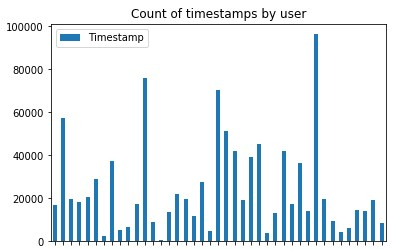
\includegraphics[width=7cm, keepaspectratio,]{fig002.jpg}
	\caption{}
	\label{fig:fig2}
\end{figure} 


\subsection{Outlier analysis} 


\section{Bayesian Inference}

Here we apply a counting process


\section{How to cite references in Latex}
\parencite{Reference1}

\medskip

This document is an example of \texttt{thebibliography} environment using 
in bibliography management. Three items are cited: \textit{The \LaTeX\ Companion} 
book \cite{latexcompanion}, the Einstein journal paper \cite{einstein}, and the 
Donald Knuth's website \cite{knuthwebsite}. The \LaTeX\ related items are
\cite{latexcompanion,knuthwebsite}. 

\medskip
